\chapter{Inferenza di Alberi Tumorali tramite Particle Swarm Optimization}
\label{chap:pso}
In questa sezione verrà descritto lo strumento di inferenza di alberi tumorali tramite Particle Swarm Optimization (d'ora in poi \textbf{PSO}), le ipotesi effettuate, i risultati ottenuti ed eventuali conclusioni. Viene utilizzata la tecnica euristica Particle Swarm Optimization, descritta precedentemente nel \autoref{chap:intro-optim-pso}.

\section{Strumenti Utilizzati}
Lo strumento è stato sviluppato in Python. Inizialmente si era cercato di utilizzare Cython\footnote{Un linguaggio di programmazione simile a Python, ma con il vantaggio di avere velocità simili a quelle ottenute da C}, poi abbandonato poiché lo studio di questo linguaggio di programmazione avrebbe ridotto il tempo utile alla vera e propria implementazione dello strumento. Si pensa però in futuro di riscrivere il codice utilizzando \textit{C++}.

L'ambiente di sviluppo scelto è \textit{Visual Studio Code}, con l'ausilio delle estensioni di debugging per Python. In generale sono sempre stati utilizzati strumenti che seguono la filosofia \textit{Open Source}, di conseguenza questa tesi ed il codice sviluppato saranno entrambi disponibili liberamente sul profilo GitHub \cite{mygithub} del sottoscritto sotto licenza GPL3 e MIT rispettivamente.

I moduli e le librerie Python che sono state utilizzate sono elencate di seguito: \begin{itemize}
  \item \pyref{random} -- modulo standard che implementa funzioni per la generazione di numeri pseudo-randomici
  \item \pyref{multiprocessing} -- modulo standard utilizzato per implementare il supporto di parallelizzazione e gestione della concorrenza
  \item \pyref{sys} -- modulo standard per accedere ad alcune variabili o funzioni di sistema
  \item \pyref{time} -- modulo standard usato per accedere a funzioni relative al tempo, come l'accesso all'ora attuale, o per la misurazione dei tempi di esecuzione
  \item \pyref{math} -- modulo standard che permette l'accesso a funzioni ottimizzate per il calcolo matematico
  \item \pyref{copy} -- modulo standard utilizzato per copiare in profondità degli oggetti, con un nuovo puntatore all'oggetto
  \item * \pypi{graphviz} -- modulo esterno per la visualizzazione ed il salvataggio su file dei grafi da formato graphviz\footnote{Strumento che permette di disegnare rappresentare dei grafi utilizzando la notazione DOT, un linguaggio che descrive la struttura di grafi generici}
  \item * \pypi{ete3} -- modulo esterno utilizzato come base di appoggio per le funzioni essenziali relative ai nodi di un albero, come la ricerca dei nodi e l'aggiunta o rimozione di essi
  \item * \pypi{networkx} -- modulo esterno sfruttato per il calcolo del \textit{maximum weight matching}
\end{itemize}

\small * Moduli esterni

\subsection{Dati utilizzati}
Per poter testare l'algoritmo ed il codice sviluppato su di esso è essenziale avere dei dati sia veri che simulati. A questo proposito sono stati utilizzati i dati simulati dal laboratorio di appartenenza del progetto, AlgoLab. Nelle seguenti sezioni verranno analizzati i dati relativi al file simulato presente nella directory del progetto \texttt{data/simulatex/exp1/sim1\_scs.txt}.
% TODO: spiegare perché è utile avere sia dati veri che simulati

\section{Adattamento del problema a Particle Swarm Optimization}
\label{chap:pso-adapt}
Una delle principali sfide in questo progetto è stata di riuscire a trovare un'interpretazione valida ed efficacie adatta alla tecnica euristica scelta, appunto il Particle Swarm Optimization, il cui funzionamento ed algoritmo sono descritti dettagliatamente nella \autoref{chap:intro-optim-pso}. Il modello più immediato da adattare al problema è quello di associare una particella dello swarm ad un albero sul quale vengono effettuate delle operazioni. Queste operazioni saranno ciò che determina il ``movimento'' della particella nello spazio. Lo swarm non è quindi altro che l'insieme degli alberi. Possiamo dividere l'implementazione in quattro fasi: \begin{enumerate}
  \item Inizializzazione
  \item Calcolo del movimento della particella
  \item Aggiornamento della particella
  \item Aggiornamento della particella migliore dello swarm e della soluzione migliore della particella
\end{enumerate}

\subsection{Inizializzazione}
\label{chap:pso-adapt-init}
Possiamo considerare una particella dello swarm come un albero, la cui posizione è determinata dalla configurazione dei suoi nodi. L'inizializzazione viene effettuata randomizzando la topologia di un albero binario $T$ con $m$ nodi, uno per ogni mutazione, con una funzione randomica\footnote{In realtà la funzione è del tipo pseudo-randomica, utilizzando il generatore \textit{Mersenne Twister} \cite{Matsumoto:MersenneTwister}, ma non avendo problemi dal punto di vista della sicurezza o della riproducibilità, è stato pervenuto che per i nostri scopi è più che valido e sufficiente}. In questo modo, viene ottenuta una topologia simile a quella rappresentata nella \autoref{fig:pso-adapt-init-topology}. Il metodo di generazione dell'albero binario è ripreso da quello implementato su SASC, ed è descritto nell'\autoref{algo:pso-adapt-init}.

\begin{algorithm}[!h]
    $m = $ numero di mutazioni
    $r = $ radice dell'albero \\
    $tree = [1, \dots, m]$ \Comment{Vettore con tutti i nodi dell'albero}
    random.shuffle(tree) \Comment{Il vettore dei nodi viene randomizzato}
    $nodes \gets [r]$ \\
    $append\_node \gets 0$ \\
    \While{$i < m$}{
      newNode $\gets$ new Node(name $=$ mutation\_name(m), parent $=$ nodes[append\_node], mutationid $=$ tree[i]) \\
      nodes.append(newNode) \\
      $i \gets i + 1$ \\
      \If{$i < m$}{
        newNode $\gets$ new Node(name = mutation\_name(m), parent = nodes[append\_node], mutationid = tree[i]) \\
        nodes.append(newNode)
      }
      append\_node $\gets$ append\_node $+ 1$
      $i \gets i + 1$
    }
    \Return{r}
    \caption{RandomTreeInit}
    \label{algo:pso-adapt-init}
\end{algorithm}

\begin{figure}[!h]
  \centering
  \begin{forest}
      germline
      [{germline}
      [{6} 
      [{18} 
      [{28} 
      [{11}  ]
      [{8}  ] ]
      [{24} 
      [{21}  ]
      [{14}  ] ] ]
      [{10} 
      [{30} 
      [{9}  ]
      [{17}  ] ]
      [{29} 
      [{1}  ]
      [{3}  ] ] ] ]
      [{23} 
      [{27} 
      [{20} 
      [{19}  ]
      [{16}  ] ]
      [{15} 
      [{12}  ]
      [{13}  ] ] ]
      [{2} 
      [{26} 
      [{7}  ]
      [{22}  ] ]
      [{4} 
      [{25}  ]
      [{5}  ] ] ] ]]
    \end{forest}    
  \caption{Esempio di topologia iniziale con $m = 30$}
  \label{fig:pso-adapt-init-topology}
\end{figure}

\subsection{Calcolo del movimento della particella}
\label{chap:pso-adapt-calculate}
La seconda fase è il calcolo della velocità con la quale una particella si muove rispetto a $p_i$ e $g$, cioè l'albero migliore che ha avuto la particella fino ad ora, e l'albero migliore in tutto lo swarm. Come parametro di paragone è definita la likelihood logaritmica descritta nell'\autoref{eq:art-sasc-lh}.

Questo step è stato uno dei problemi principali da affrontare sin dal principio del progetto. Non è immediato trovare un modello diretto che rappresenti la velocità e la direzione di una particella verso gli alberi migliori $p_i$ e $g$, data la natura non lineare del problema. Sono state, dunque, introdotte diverse metriche (o assenza di tali) per cercare di definire al meglio questo parametro in maniera tale che aderisse al meglio all'algoritmo scelto, quindi PSO. Nelle seguenti sottosezioni verranno descritti tali esperimenti, con risultati e considerazioni del caso.

\subsubsection{Assenza del parametro di velocità}
\label{chap:pso-adapt-calculate-1}
Nei momenti iniziali di questo progetto, come è stato descritto precedentemente, trovare una corrispondenza congeniale ed adeguata all'idea di \textit{velocità} del PSO è stato impegnativo. Al fine comunque di poter dare un via al lavoro, una delle prime metriche adottate di velocità è stata la vera e propria assenza di tale metrica. I risultati descritti nella \autoref{fig:pso-adapt-calculate-1-table} possono sembrare promettenti, dato che comunque provano la funzionalità del programma, e che la likelihood aumenta. Quello che i dati non ci dicono è però qualcosa che possiamo intuire dall'intrinseco comportamento dell'assenza della velocità come metrica: siamo di fronte ad un semplice algoritmo di highest hill climbing, descritto nella \autoref{chap:intro-optim-hill}. Quello che succede quindi è che si cerca di migliorare l'algoritmo al primo miglioramento individuato, in questo caso corrisponde ad ogni volta che si trova una likelihood migliore. Questo può sembrare un ottimo risultato, ma è in realtà un problema. L'estrema e ripida scalata rischia di incastrare la ricerca in un ottimo locale, peggiorando considerevolmente le possibilità di trovare un albero filogenetico di \textbf{buona qualità}. È importante sottolineare la \textit{bontà} del risultato, e non il basso valore della \textit{likelihood}, in quanto questo è solo un valore indicativo della verosomiglianza dell'albero con i dati a nostra disposizione, ma non dell'effettiva qualità della loro rappresentazione. È molto meglio quindi cercare di trovare un albero filogenetico con una qualità migliore che quello con la likelihood più elevata.

\begin{figure}[!h]
  \centering
  \begin{tabular}{*{5}{c}}
    Particelle & Iterazioni & Likelihood Iniziale & Likelihood Migliore & Tempo Impiegato (s) \\ \midrule \midrule
    5 & 20 & -8865.285307 & -8029.856799 & 19.102292 \\
    10 & 20 & -8865.285307 & -8002.707585 & 33.599134 \\
    50 & 20 & -8341.992690 & -6296.678757 & 179.630704 \\
    85 & 20 & -8341.992690 & -6804.514080 & 296.845929 \\
    100 & 20 & -8341.992690 & -6260.733733 & 351.863327 \\
    150 & 20 & -8163.910048 & -6341.065027 & 536.725522 \\
    200 & 20 & -7944.950318 & -6897.161794 & 737.740094
  \end{tabular}
  \caption{Risultati ottenuti con assenza della velocità}
  \label{fig:pso-adapt-calculate-1-table}
\end{figure}
\begin{figure}[!h]
  \centering
  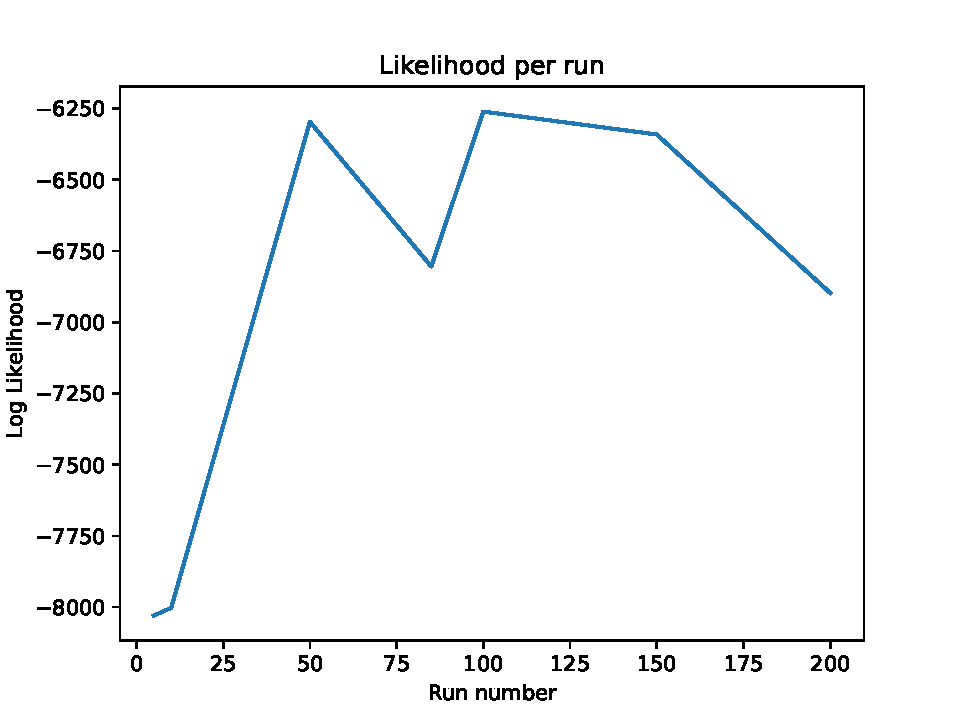
\includegraphics[width=0.8 \textwidth]{322_lh_no_velocity.pdf}
  \caption{Grafico della likelihood sui vari parametri delle particelle con l'assenza della velocità}
  \label{fig:pso-adapt-calculate-1-graph}
\end{figure}

\subsubsection{Velocità come numero di nodi presi dall'albero migliore}
% TODO:

\section{Modello degli errori single-cell}
\label{chap:pso-matrix}
I dati single-cell vengono rappresentati tramite un modello di sostituzione come quello illustrato nella \autoref{chap:intro-models} tramite una matrice $M = n \times m$, con $n$ cellule e $m$ mutazioni. Viene poi utilizzata una matrice $D = n \times m$ è ricavata dall'osservazione dell'albero inferito, ed è una versione imperfetta del vero genotipo della matrice $M$. Per mitigare i problemi causati dalle tecniche di WGA (\autoref{chap:intro-scs}) viene utilizzato il parametro $\alpha$ per indicare la probabilità di incontrare un falso positivo, quindi osservare un $1$ quando in realtà questo è uno $0$, e falsi negativi, cioè di avere la probabilità $\beta$ di osservare uno $0$ quando in realtà è un $1$:
\begin{align}
    \label{eq:pso-intro-model-matrix}
    \begin{split}
      P(M_{i,j} = 0 | D_{i,j} = 0) = 1 - \alpha, \qquad
      &P(M_{i,j} = 0 | D_{i,j} = 1) = \beta, \\
      P(M_{i,j} = 1 | D_{i,j} = 0) = \alpha, \qquad
      &P(M_{i,j} = 1 | D_{i,j} = 1) = 1 - \beta
    \end{split}
\end{align}

\section{Considerazioni aggiuntive}
Al fine di poter eseguire delle anlisi e considerazioni sui risultati ottenuti sono stati fatti diversi accorgimenti sul progetto, di seguito analizzati.

\subsection{Riproducibilità}
Durante lo sviluppo di un software può capitare di dover rappresentare una situazione, come un bug, una feature, o un risultato particolare. Questa necessità dà luogo al problema della \textit{riproducibilità}, che implica la possibilità allo sviluppatore o a terzi di poter eseguire il software con parametri comuni al fine di ottenere gli stessi risultati e situazioni. Questo obiettivo è stato raggiunto con diversi accorgimenti, come l'elevata flessibilità di configurazione da linea di comando (descritta in dettaglio nel \autoref{chap:pso-extra-guide}) e la possibilità di poter manipolare gli eventi aleatori fissando un \textit{seed}\footnote{Un numero, o vettore, utilizzato per inizializzare un generatore pseudo-casuale di numeri, come quello utilizzato dalla libreria \textit{random} di Python}.

\subsection{Guida allo strumento nello stato attuale}
\label{chap:pso-extra-guide}

\subsection{Parallelizzazione}

\section{Risultati e conclusioni}

\section{Prospettive future}
